\documentclass[12pt]{article}

\usepackage{graphicx}
\usepackage{hyperref}
\graphicspath{ {./img/} }
\usepackage{tikz}


\begin{document}
\newcommand{\reporttitle}[2]{
\center
\rule[0.2cm]{13cm}{0.1cm}
{ \huge \bfseries #1}\\[0.4cm] % Title of your document
{\Large \slshape #2}\\[0.4cm]
\rule[0.2cm]{13cm}{0.1cm}\\[3cm]
}

\newcommand{\UNI}{
\textsc{\Huge TEZPUR \\[0.3cm] University}\\[0.7cm]
}

\newcommand{\info}[2]{
\begin{minipage}{0.4\textwidth}
\normalsize
\centering
#1 \textsc{#2}\\
\end{minipage}\\
}

\begin{titlepage}

\center 
\UNI

\reporttitle{Environmental Law Survey}{A survey project on Environmental Law Awareness}

\info{Name: } {AMAN KUMAR}
\info{Roll: } {EEB20035}
\info{Department: } {Electrical Engineering}
\vfill

\end{titlepage}
\newpage
\begin{titlepage}
    \begin{center}
        \textbf{{\Huge CERTIFICATE}}
    \end{center}
    
    \noindent    
{\Large This  is  to  certify  that  Aman Kumar,  B.tech  3rd  Semester 
student in the Department of Electrical Engineering, Tezpur  University  has  completed  his  project  titled  \emph{Environmental Law Survey : A survey project on Environmental Law Awareness}  under 
our supervision. 
On the basis of his work, we certify that no similar work has been ever 
carried out on this subject earlier with the same title anywhere. }
\\ \\ \\ \\ \\ \\
\\ \\ \\ \\ \\ \\

\noindent
{\Large Dr. Madhumita Ghosh Datta and Dr. Nazrin Ullah \\
Department of Environmental Science \\
Tezpur University \\}
\end{titlepage}
\newpage
\begin{titlepage}
    \begin{center}
        \textbf{{\Huge ACKNOWLEDGEMENT}}
    \end{center}
    \noindent
{\Large It  gives  me  immense  pleasure  to  express  my  gratitude  towards  our 
Course  Instructors  for  Environmental  Studies,  Dr.  Madhumita  Ghosh Datta and Dr. Nazrin Ullah  for  their  guidance,  support  and  encouragement  throughout  the 
duration of the project. Without their help and motivation, the 
successful  completion  of  this  project  would  not  have  been  possible. I
would also like to thank my family members and friends without whose support, it 
would have been impossible to complete the project.}
\end{titlepage}
\newpage
\section{ Introduction }
Environmental law is a collective term encompassing aspects of the law that provide protection to the environment.A related but distinct set of regulatory regimes, now strongly influenced by environmental legal principles, focus on the management of specific natural resources, such as forests, minerals, or fisheries. Other areas, such as environmental impact assessment, may not fit neatly into either category, but are nonetheless important components of environmental law.
\\ \\
The need for protection and conservation of environment and sustainable use of natural resources is reflected in the constitutional framework of India and also in the international commitments of India. The Constitution under Part IVA (Art 51A-Fundamental Duties) casts a duty on every citizen of India to protect and improve the natural environment including forests, lakes, rivers and wildlife, and to have compassion for living creatures. Further, the Constitution of India under Part IV (Art 48A-Directive Principles of State Policies) stipulates that the State shall endeavour to protect and improve the environment and to safeguard the forests and wildlife of the country.
\\ \\
However these environment laws aren't too common for the general public and this study aims to study the Environmental Law Awareness around a locality. 

\section{Methodology}
The study attempts to find about  the perception of people in our town or village 
on Environmental Laws. The  quantitative  part  of  the  study  was  done  through 
Google  Forms,  which  was  circulated  randomly  among 51 households of  the  locality (Dhanbad , Jharkhand) 
mainly  via  WhatsApp. The  responses  were  collected  between  the  period  of  20th 
September,  2021,  and  12th  October,  2021.  The  collected  data  was  then 
analyzed and presented. 

\newpage
\section{Results}
A total of 51 people responded to the survey, out of which the 27.5\% were females, 68.6\% were males while remaining 3.9\% chose to not disclose their gender. 
98\% of the respondents belonged to the age group of '15-25 years', while 2\% belonged to the age group of '30-50' years. In terms of educational qualifications, around 
54.9\% are 12th pass, followed by 25.5\% graduates and 13.7\% post graduates. 
\\ \\ \noindent
When asked about local or national environmental laws, only 35.3\% claim to know them while 27.5\% deny and 37.3\% are not sure about it.
\\
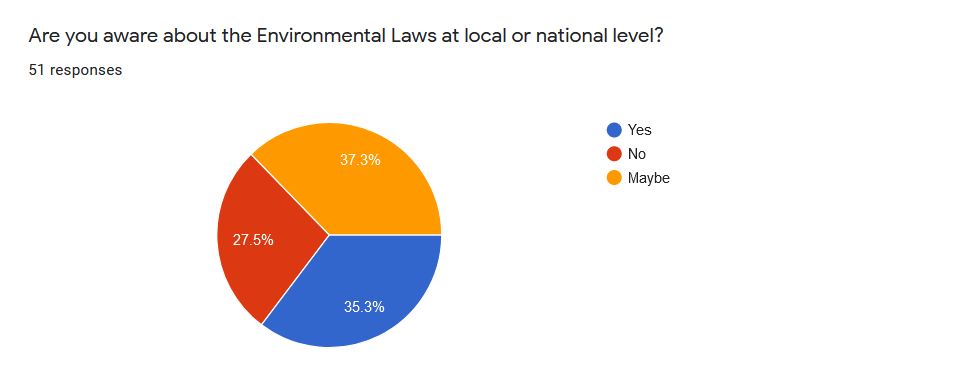
\includegraphics[scale=1]{1}
 \\ \\ 
 On being asked to rate the neccesity of environmental laws on a scale of 1-5, around 68.6\% strongly agreed, rating it 5, while 15.7\% and 15.7\% people rated it 4 and 3 respectively. 
 The people who strongly disagreed  or disagreed with the neccesity of environmental laws were 0\%. 
\\ 
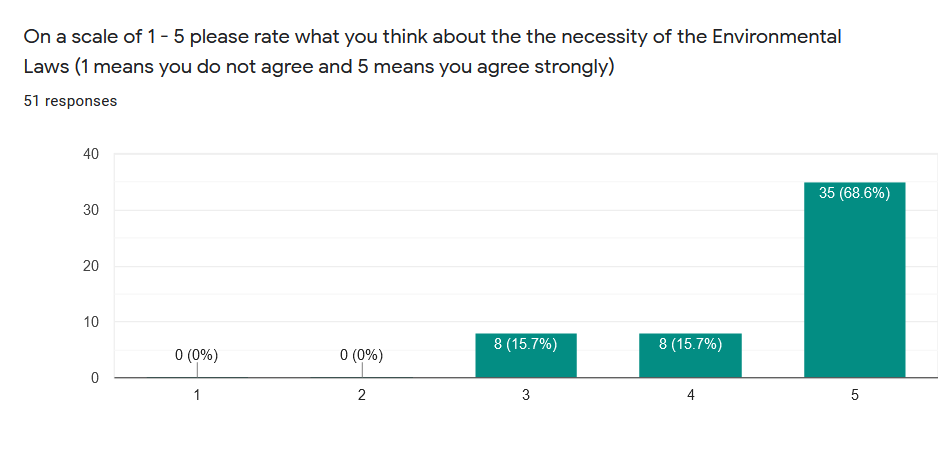
\includegraphics[scale=0.7]{2}
\\ \\
On being asked if the existing environmental laws are enforced correctly, 78.4\% of the respondents disagree, while 17.6\% of the respondents are not sure about it, followed by 3.9\% people responding to it positively.
\\ \\
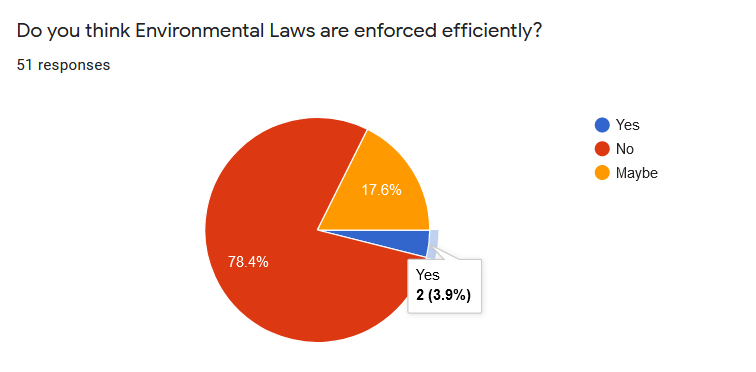
\includegraphics[scale=1]{3}
\\ \\
A total of 84.3\% of respondents deny when asked, if they ever got themselves into trouble because of non compliance of Environmental Laws. While 7.8\% and 7.8\% respond in yes and maybe respectively.
\\ \\
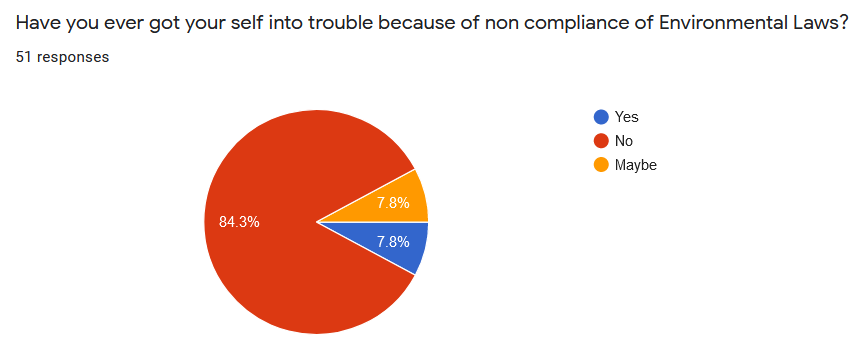
\includegraphics[scale=0.8]{4}
\\ \\
A total of 58.8\% of respondents try to follow environmental laws conciously, while rest are either not sure about it or just don't bother following the laws. 
\\ \\ 
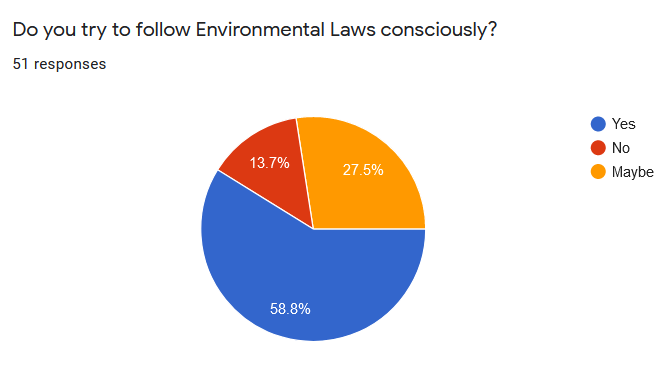
\includegraphics[scale=0.8]{5}
\\ \\
When asked about, how they feel about the statement "Monetary Penalties for violation of Environmental Laws is good.", we get a variety of responses. 
37.3\% of the respondents strongly agree while 7.8\% of the respondents disagree. While majority lies with the mildly agree or agree. 
\\ \\ 
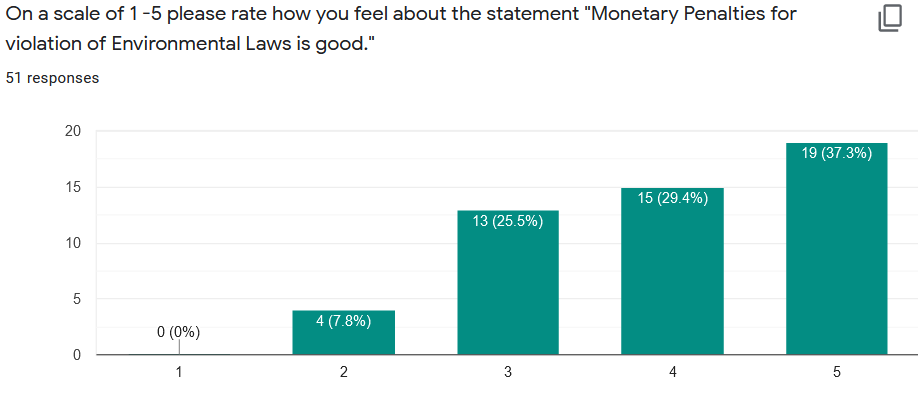
\includegraphics[scale=0.7]{6}

\section{Conclusion}

Despite so much of effort being put on the awareness of Environmental Laws  
and holding programs on it, very little have actually been actually
realized.
\\ \\
\noindent
Most people are still unaware about the Environmental Laws and are not conciously thinking about following the laws even if they are aware about them. This trend was visible in the data, irrespective of the educational qualifications of the individuals. 
Highly educated and not so highly educated are both equally ignorant about the laws. 
\\ \\ 
\noindent
A lot is required to be done in order to make people aware and follow the environmental laws. The laws and plans written on the papers are to be brought to the people by properly implimenting them for the sake of humans and nature. 


\section{References}
\begin{enumerate}
    \item \url{https://en.wikipedia.org/wiki/Environmental_law}
    \item \url{https://www.britannica.com/topic/environmental-law}
    \item \url{https://www.mondaq.com/india/waste-management/624836/environment-laws-in-india}
\end{enumerate}
\end{document}
